\section{Speech Act}
\subsection{Speech Act}
\begin{frame}{Speech Act}

    We could also  use Speech Act to make the conversation more robust and human-like by using them as features.
    \vspace{3mm}

    Each utterance in a dialog is closely related to an action. Speech acts refer to the various functions that language can perform beyond conveying information
    \begin{itemize}
        \item \textbf{Assertives}: Statements that convey information.
\item \textbf{Directives}: Commands or requests.
\item \textbf{Commissives}: Promises, commitments.
\item \textbf{Expressives}: Expressions of emotion or attitude.
\item \textbf{Declarations}: Changes the state of affairs
\item \textbf{Acknowledgements}

    \end{itemize}

    Thus speech act expresses an important component of the intention of the spoken/written sentences
\end{frame}

\begin{frame}[fragile]{Locutionary act}
            This basic level of communication focuses on the literal meaning conveyed by the words themselves

    \begin{block}{Examples}

    \begin{itemize}
        \item Coveys directly the  literal meaning
        \item Doesn't involve intention, context, or interpretation

      \item Essential for building more complex speech acts.
        \begin{itemize}
            \item  \verb|The sky is blue| - simple statement
            \item \verb|What time is it?| - question $\smile$
            \item \verb|Stop| - commands
            \item \verb|Congratulations|- Exclamations
            \item \verb|I promise|- Performatives
        \end{itemize}
    \end{itemize}
    \end{block}
\end{frame}
\begin{frame}[fragile]{illocutionary act}

    Each of these sentences not only conveys information but also performs a particular illocutionary act, such as expressing a belief, making a request, committing to an action, expressing emotions, or making a declaration.
    \begin{block}{Examples}
     \begin{itemize}
         \item \verb|I believe that the sky is blue |- assertive
         \item  \verb|Please pass the salt| - Directive
         \item \verb|I promise to meet you at 5 pm| - Commissive
         \item \verb|Congratulations on your promotion! |- Expressive
         \item  \verb|I declare this meeting adjourned |- Declarative
     \end{itemize}
    \end{block}
\end{frame}

\begin{frame}{Speech Act with examples}
    \begin{figure}
        \includegraphics[width=0.7\linewidth]{Images/speech_Act_Example}
        \label{fig:speechactexample}
    \end{figure}
    Source: \href{https://web.stanford.edu/class/linguist130a/2022/materials/ling130a-handout-03-08-speechacts.pdf}{Speech Act}
\end{frame}


\begin{frame}{Key Evaluation Metrics}
\begin{itemize}
    \item Essential for comparing QA system implementations
    \item Primary metrics (Yao, 2014):
    \begin{itemize}
        \item Accuracy
        \item F1 Score
    \end{itemize}
\end{itemize}
\end{frame}

\begin{frame}{Contingency Table Basis}
\begin{table}
\centering
\begin{tabular}{lcc}
\hline
 & \textbf{Actual Positive} & \textbf{Actual Negative} \\
\hline
\textbf{Predicted Positive} & True Positive (TP) & False Positive (FP) \\
\textbf{Predicted Negative} & False Negative (FN) & True Negative (TN) \\
\hline
\end{tabular}
\end{table}
\end{frame}

\begin{frame}{Accuracy}
\[
\text{Accuracy} = \frac{TP + TN}{TP + FP + FN + TN}
\]

\begin{itemize}
    \item Challenge in QA systems:
    \item High TN rates can inflate accuracy scores
    \item Particularly problematic for fact-based questions
\end{itemize}
\end{frame}

\begin{frame}{Precision vs Recall}
\begin{columns}
\begin{column}{0.5\textwidth}
\textbf{Precision}
\[
P = \frac{TP}{TP + FP}
\]
\begin{itemize}
    \item Focus: Correctness of selected answers
    \item Preferred for definition/list QA
\end{itemize}
\end{column}

\begin{column}{0.5\textwidth}
\textbf{Recall}
\[
R = \frac{TP}{TP + FN}
\]
\begin{itemize}
    \item Focus: Completeness of correct answers
    \item Preferred for fact-based QA
\end{itemize}
\end{column}
\end{columns}
\end{frame}

\begin{frame}{F1 Score: Balanced Metric}
\[
F1 = \frac{2 \times P \times R}{P + R}
\]

\begin{itemize}
    \item Harmonic mean of precision and recall\cite{kumar2019}, \cite{yao2014information}, \cite{zhou2013improving}
    \item Addresses precision-recall trade-off
    \item Preferred for systems requiring balance
\end{itemize}

\end{frame}

\begin{frame}{Metric Selection Guidelines}
\begin{itemize}
    \item \textbf{Recall-focused:}
    \begin{itemize}
        \item Fact-based QA systems
        \item High TP critical
    \end{itemize}

    \item \textbf{Precision-focused:}
    \begin{itemize}
        \item Definition/list QA systems
        \item Minimizing FP essential
    \end{itemize}

    \item \textbf{F1 Score:}
    \begin{itemize}
        \item When balance between P \& R needed
        \item General system comparisons
    \end{itemize}
\end{itemize}
\end{frame}


%\begin{frame}{Grounding}
%    Any dialog is not an independent set of sentences. Dialogs happen on a \textbf{\underline{common ground}}. The speakers often perform ground Grounding act by acknowledging that the hearer has understood the speaker
%\end{frame}